% !TeX program = xelatex
\documentclass[12pt, twoside]{report}

% Packages
\usepackage{amsfonts,amsmath,amsthm}
\usepackage[utf8]{inputenc}
\usepackage[T1]{fontenc}
\usepackage{graphicx}
\usepackage{fontspec}
\usepackage[a4paper, width=150mm, top=25mm, bottom=25mm, bindingoffset=6mm]{geometry}
\usepackage{fancyhdr}
\usepackage[hidelinks]{hyperref}
\usepackage{nameref}
\usepackage[style=numeric, citestyle=authortitle]{biblatex}
\usepackage{algorithm,algcompatible}
\usepackage[noend]{algpseudocode}
\usepackage{algorithmicx}
\usepackage{float}
\usepackage{adjustbox}

%% Fonts
% main
\setmainfont{UT Sans}[
UprightFont=*-Regular,
BoldFont=*-Medium,
ItalicFont=*-Regular,
ItalicFeatures={FakeSlant=0.3},
BoldItalicFont=*-Medium,
BoldItalicFeatures={FakeSlant=0.1},
]
% algorithms
\newfontfamily{\algfont}{Courier}
\let\algorithmicOLD\algorithmic
\def\algorithmic{\algorithmicOLD\algfont}

% Header & Footer
\pagestyle{fancy}
\fancyhead{}
\fancyhead[LO,RE]{Manghiuc Teodor-Adrian \\ Informatică Aplicată}
\fancyhead[RO,LE]{Universitatea Transilvania \\ Facultatea de Matematică și Informatică}
\fancyfoot{}
\fancyfoot[LE,RO]{Pag. \thepage}
\renewcommand{\headrulewidth}{0.4pt}
\renewcommand{\footrulewidth}{0.4pt}
\renewcommand{\figurename}{Fig.}
\renewcommand{\chaptername}{Capitolul}
%\rhead{Manghiuc Teodor-Adrian \\ Informatică Aplicată}
%\lhead{Universitatea Transilvania \\ Facultatea de Matematică și Informatică}

% Disables paragraph indentation
\setlength{\parindent}{0pt}

% Graphics path
\graphicspath{ {Images} }

% Biblatex References
\addbibresource{references.bib}

% Algorithm comments
\renewcommand{\COMMENT}[2][.5\linewidth]{%
	\leavevmode\hfill\makebox[#1][l]{~#2}}

% General info
\title{Lucrare de licență}
\author{Manghiuc Teodor-Adrian}
\date{}

% Document
\begin{document}
	\begin{titlepage}
	\begin{center}
		
\includegraphics[width=240pt]{./Images/Logo/Logo-UT-MI-RGB-EN}
		\vspace*{48pt}\\
		\textbf{\LARGE Lucrare de licență}
		\vspace*{12pt}\\
		\LARGE FoodSpy\\
		\large Aplicație web pentru gestiunea aportului zilnic de calorii
		\vspace*{48pt}\\
		\begin{center}
			\large
			\begin{tabular}{ll}
				\textbf{Autor:}&Manghiuc Teodor-Adrian\\
				%\textbf{Mentor:}&\\
				\textbf{Coordonator:}&Monescu Vlad\\
			\end{tabular}
		\end{center}
		
		\vfill
		\large Brașov, România\\2020-2021
	\end{center}
\end{titlepage}
	
	\chapter*{Abstract}
	
	\chapter*{Mențiuni}
	
	\tableofcontents
	
	\chapter{Introducere}
	%\input{chapters/00_Introduction}
	
	\chapter{Aplicații web - noțiuni teoretice}
	%\input{chapters/01_TheoreticalTerms}
	
	\chapter{Limbaje de programare}
	% !TeX root = ../FoodSpy.tex
% \section{Limbaje de programare}

\section{JavaScript / TypeScript}
JavaScript este un limbaj de programare care permite implementarea unor funcționalități complexe în paginile web. Câteva dintre aceste funcționalități sunt actualizarea conținutului paginilor web în mod dinamic, animarea de grafice 2D sau 3D și afișarea hărților interactive. Alături de HTML și CSS, JavaScript este unul dintre tehnologiile web standard.
\\ \\
JavaScript este un limbaj multi-platformă, poate fi folosit pe partea de client, dar și pe partea de server, este ușor de învățat și este dinamic și flexibil. Această dinamicitate este însă și unul din dezavantajele limbajului. De exemplu, JavaScript pune la dispoziție variabile primitive de tip ”string” sau ”number”, dar pentru că nu este necesară compilarea codului, nu se verifică folosirea corectă a acestor variabile, programatorul putând folosi o variabilă ”title” pentru a reține un ”string” (Fig. \ref{fig:31}), dar care mai târziu poate va fi suprascrisă și se poate reține (în variabilă) un ”number”, fără niciun fel de avertizare din partea mediului de programare, putând conduce la bug-uri și la comportamente neprevăzute.

\begin{figure}[!htb]
	\centering
	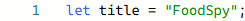
\includegraphics
	{../LaTeX/Images/ts_title-1.PNG}
	\caption{Definirea variabilei ”title”}
	\label{fig:31}
\end{figure}

Aici intervine TypeScript, un superset al limbajului JavaScript ce adaugă ”siguranța de tip” necesară pentru evitarea situațiilor neplăcute precum este cea descrisă mai sus. TypeScript încurajează scrierea codului în stil declarativ, asemănător limbajelor C\# sau Java prin facilități ca interfețe, clase și inferența de tip a variabilelor.
\\ \\
Este necesară compilarea codului scris în limbaj TypeScript, dar acest lucru poate fi văzut ca un avantaj pentru că mediul de programare poate astfel scoate în evidență comportamentul neașteptat al codului și prin urmare poate duce la detecția mult mai rapidă a bug-urilor. Referindu-ne la situația neplăcută descrisă mai sus, dacă variabila ”title” ar fi adnotată cu tipul ”string”, atunci nu va putea fi suprascrisă de o valoare pretabilă unei variabile de tip ”number”.
\newline

\begin{figure}[!htb]
	\centering
	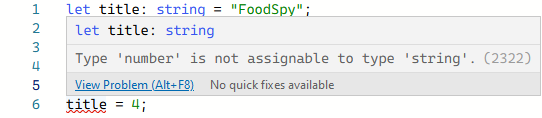
\includegraphics
	{../LaTeX/Images/ts_title-2.PNG}
	\caption{Adnotarea previne suprascrierea variabilei ”title”}
	\label{fig:32}
\end{figure}

TypeScript vine în ajutorul programatorilor care sunt deja obișnuiți cu limbaje de programare cu stil declarativ și propune astfel o alternativă față de JavaScript care nu oferă niciun suport pentru ”siguranța de tip”.
\\ \\
Deși o mai bună înțelegere a limbajului JavaScript este recomandată, TypeScript se poate învăța și folosi în mod independent, fără a cunoaște toate dedesubturile JavaScript. Mai mult, un bonus pentru programatorii cu experiență în C\# este faptul că autorul limbajului TypeScript este arhitectul limbajului C\#, deci, din punct de vedere sintactic, TypeScript și C\# împărtășesc multe similitudini.

\begin{figure}[htbp]
	\centering
	%\hspace*{-2cm}
	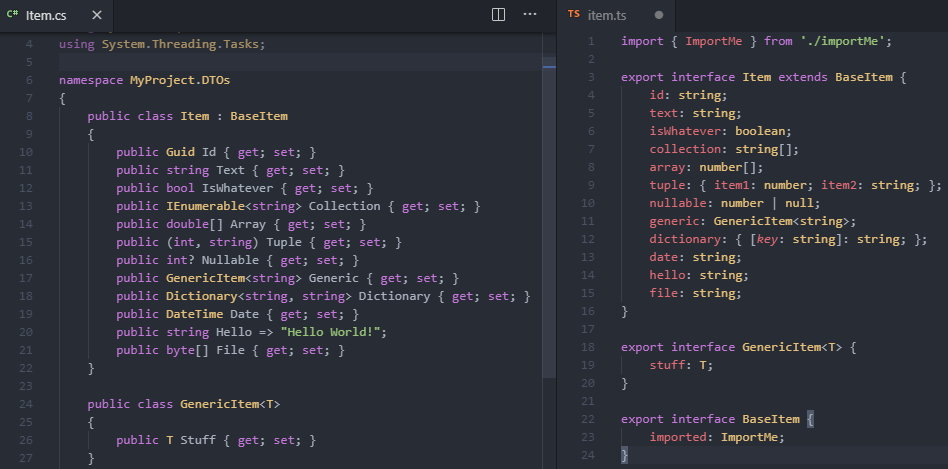
\includegraphics[width=1\textwidth]
	{../LaTeX/Images/ts_similar-3.PNG}
	\caption{Asemănări între C\# și TypeScript}
	\label{fig:33}
\end{figure}

Față de JavaScript, TypeScript întinde o plasă de siguranță care poate prinde defectele de programare introduse prin modificări majore ale codului. TypeScript nu va înlătura necesitatea depanării programelor, dar ”siguranța de tip” va ajuta fără echivoc la detectarea din timp ale defectelor. Mai mult, TypeScript beneficiază de sugestii și avertizări din partea mediului de programare încă de la compile-time, în timp ce erorile în JavaScript pot fi descoperite abia la run-time.
\\ \\
Printre alte avantaje ale TypeScript includem și posibilitatea re-factorizării într-un mod mai sigur deoarece se cunoaște codul la nivel semantic și capabilitățile TypeScript care permit construirea aplicațiilor de mărime foarte mare, în completă antiteză cu JavaScript care a fost gândit ca un limbaj folosit strict pentru modificarea dinamică a paginilor web.


\section{C\#}
C\# este un limbaj de programare orientat pe obiect, simplu, dar puternic și este gândit pentru dezvoltarea de aplicații pe platforma .NET Framework. Moștenește părțile bune ale limbajului C++ și Visual Basic, dar fără anumite inconsistențe \footnote{O astfel de inconsistență în C++ este accesul la un element dintr-un ”std::vector”. În C++ se poate folosi operatorul ”[]” pentru a ajunge la elemente care nu sunt de fapt elementele ale vectorului, ci sunt bucăți de informație conținute la adresele de memorie adiacente memoriei alocate vectorului. Deoarece nu se face niciun fel de verificare a indicelui elementului pe care încercăm să-l accesăm, operatorul ”[]” va întoarce ceea ce se află la locația de memorie vecină memoriei alocate vectorului.} și anacronisme ceea ce duc la un limbaj mai logic și mai puțin complicat.
La fel cum pentru o variabilă, simbolul ”++” înseamnă incrementarea cu 1 după ce variabila a fost evaluată, pentru C\#, simbolul ”\#” semnifică o incrementare a limbajului C++.
\\ \\
Prima versiune a apărut în 2001. Odată cu versiunea 2.0 au apărut lucrul cu generice, iteratori și metode anonime. În versiunea 3.0 au debutat metodele de extensie, expresiile lambda și cel mai important, LINQ sau Language-INtegrated Query. Versiunea 5.0 a venit cu suport nativ pentru operațiile asincron prin introducerea operatorului ”await” și modificatorului de funcție ”async”.
\\ \\
%\label{cgenerics}
Lucrul cu clase și metode generice reprezintă un concept care face posibilă proiectarea de clase și metode ale căror tipuri se cunoaște doar la momentul declarării sau instanțierii. Acest concept combină reutilizarea codului, ”siguranța de tip” și eficiența într-un mod în care nu este posibil prin proiectarea specifică.
\\ \\
”GenericList” din (Fig. \ref{fig:34}) este un exemplu de clasă generică care modelează o listă simplu înlănțuită capabilă să memoreze obiecte de tip ”Node” de orice tip, inclusiv ”int”, ”double” sau ”string”.

\begin{figure}[!htb]
	\centering
	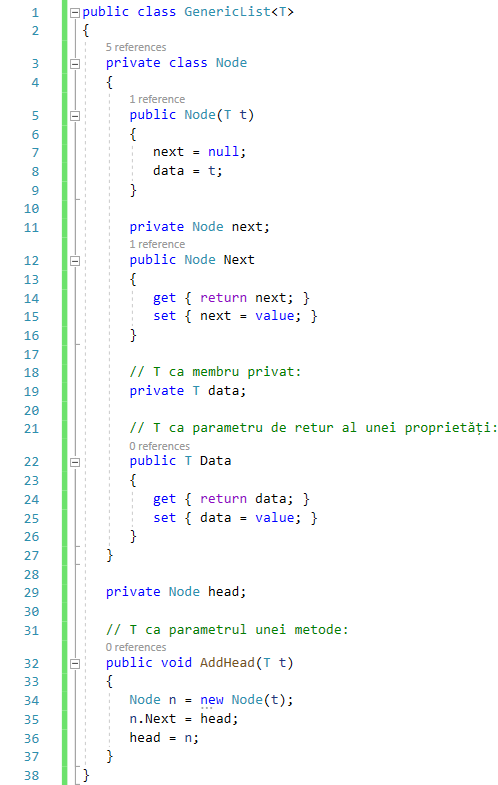
\includegraphics[width=0.8\textwidth]
	{../LaTeX/Images/csharp_generics.PNG}
	\caption{Exemplu de clasă generică}
	\label{fig:34}
\end{figure}

Parametrul de tip ”T” ia locul declarării tipului explicit și este folosit ca parametru în metoda ”AddHead(T t)”, ca parametru de retur al proprietății ”Data” și ca tip de membru privat, cum este cazul membrului ”T data”. La momentul instanțierii clasei ”GenericList<T>”, fiecare apariție a lui ”T” va fi înlocuită de tipul specificat între ”<>”.
Se pot crea interfețe, clase, metode, evenimente și delegați generici.
\\ \\
%\label{cextmeth}
Metodele de extensie sunt o funcționalitate a limbajului C\# care permit adăugarea de metode tipurilor deja existente. Metodele de extensie sunt metode statice care sunt apelate ca și cum ar fi membre ale clasei, cum este de exemplu metoda ”ToString()”, membră a clasei ”Object”.
\\ \\
O metodă de extensie are cel puțin un parametru, ”this” care reprezintă obiectul curent peste care operează metoda. Din cauza aceasta, când se apelează o metodă de extensie de către un obiect, obiectul nu trebuie trimis ca parametru.
”WordCount” din (Fig. \ref{fig:35}) este o metodă de extensie care numără caracterele dintr-un obiect de tip ”string”. Se observă că ”WordCount” este definită pentru obiecte din clasa ”System.String” deoarece parametrul ”str” este prefixat de ”this string”.

\begin{figure}[!htb]
	\centering
	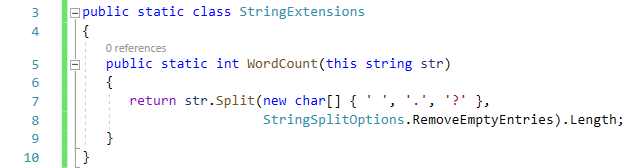
\includegraphics
	{../LaTeX/Images/csharp_extension-1.PNG}
	\caption{Exemplu de metodă de extensie}
	\label{fig:35}
\end{figure}

Apelul metodei de extensie se poate observa în (Fig. \ref{fig:36}).

\begin{figure}[!htb]
	\centering
	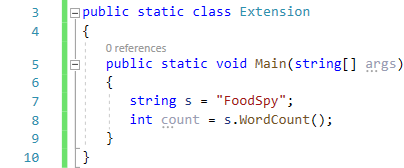
\includegraphics
	{../LaTeX/Images/csharp_extension-2.PNG}
	\caption{Apelul unei metode de extensie}
	\label{fig:36}
\end{figure}

%\label{clinq}
O definiție simplistă pentru LINQ este următoarea: modalitatea prin care se poate interoga o bază de date folosind un limbaj de interogare apropiat de SQL, dar care este compilat în interiorul unei aplicații care rulează pe platforma .NET.
Prin ”bază de date” se înțelege un spectru larg de surse de date, printre care baze de date SQL, baze de date ”in-memory” sau reprezentări XML.
\\ \\
LINQ permite scrierea unei interogări sub forma unei structuri SQL, după cum se poate observa în (Fig. \ref{fig:37}). Această structură are avantajul că variabila ”name” este ”scoped”, adică nu trebuie definită din nou pentru fiecare clauză din interogare.

\begin{figure}[!htb]
	\centering
	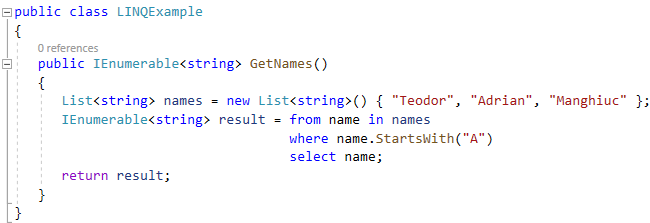
\includegraphics
	{../LaTeX/Images/csharp_linq-1.PNG}
	\caption{Exemplu de interogare LINQ}
	\label{fig:37}
\end{figure}

Un alt avantaj este claritatea originii variabilei ”name” - chiar din primul rând ("from name in names") se distinge faptul că ”name” provine din sursa de date ”names”, spre deosebire de interogarea SQL clasică, unde clauza ”from” ar fi fost declarată ultima.

LINQ nu ar fi fost un concept realizabil dacă nu s-ar fi implementat în prealabil funcționalități precum metodele de extensie, tipurile anonime \footnote{List<string> names = new List<string>() \{ "Teodor", "Adrian", "Manghiuc" \};\\Din construirea unei variabile, compilatorul are la dispoziție suficiente informații pentru a pune la dispoziție un tip de date care să modeleze variabila.}, tipurile implicite \footnote{var anonymousType = names.Select(n => new \{ Name = n, Capitalized = n.ToUpper() \});\\Din inițializarea unei variabile, compilatorul are la dispoziție suficiente informații pentru a infera tipul acesteia.\\var inference = names.Select(n => n);\\devine\\IEnumerable<string> inference = names.Select(n => n);} și expresiile lambda.


\section{HTML și CSS / SCSS}
%\label{html}
Acronimul HTML vine de la Hypertext Markup Language și reprezintă limbajul care permite structurarea conținutului unei pagini web prin construirea de secțiuni, definirea de rubrici, paragrafe și link-uri.
HTML nu este un limbaj de programare, deci nu permite construirea de conținut cu funcționalitate dinamică, dar face posibilă organizarea și formatarea paginilor web, asemenea documentelor scrise în Microsoft Word.
\\ \\
HTML este format dintr-o colecție de elemente folosite pentru a ”înfășura” bucățile de conținut astfel încât să arate sau să se comporte într-un anume fel. De exemplu, folosind elementul ”<a>” putem crea un link către o altă pagină web, cu ”<i>” putem scrie înclinat, iar cu ”<h1>” putem defini o rubrică.
În (Fig. \ref{fig:38}), este ilustrat elementul ”<p>”.

\begin{figure}[!htb]
	\centering
	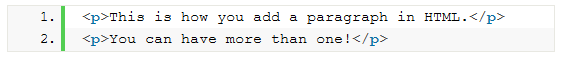
\includegraphics
	{../LaTeX/Images/html_element.PNG}
	\caption{Exemplu de element HTML}
	\label{fig:38}
\end{figure}

”p” vine de la paragraf. ”<p>” se mai numește ”opening tag” și definește punctul de intrare al elementului de tip paragraf și se poate observa că este închis între simbolurile ”<” și ”>”. ”</p>” reprezintă ”closing tag” și marchează punctul de ieșire al elementului, care, spre deosebire de punctul de intrare, mai are în componență simbolul ”/”. Textul sau conținutul paragrafului este definit între punctul de intrare și cel de ieșire. Un element HTML este format din toate cele 3 părți descrise mai sus.
\\ \\
%\label{css}
Acronimul CSS vine de la Cascading Style Sheets și reprezintă limbajul care permite determinarea aspectului unei pagini web, din punct de vedere vizual, schematic și estetic. Dacă HTML este planul unei case, CSS precizează stilul acesteia, Victorian sau Art Deco, Post-modern sau Gotic.
\\ \\
CSS schimbă aspectul paginii web interacționând cu elementele HTML. După cum am observat în (Fig. \ref{fig:38}), un paragraf este un asemenea element HTML. Dacă vrem ca textul paragrafului să fie de culoare roz și cu scris îngroșat, vom scrie codul CSS ilustrat în (Fig. \ref{fig:39}).

\begin{figure}[!htb]
	\centering
	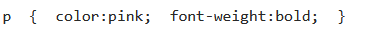
\includegraphics
	{../LaTeX/Images/css_paragraph.PNG}
	\caption{Exemplu de stilizare CSS}
	\label{fig:39}
\end{figure}

%maybe add \\ \\ here%
”p” se numește ”selector” și indică elementul HTML căruia îi vom schimba aspectul folosind reguli definite în CSS. ”color” și ”font-weight” sunt câteva dintre proprietățile de stilizare care se pot aplica selectorului de tip ”p”. Alte proprietăți ale acestuia sunt dimensiunea textului, adică ”font-size” sau ”text-transform” care poate transforma textul paragrafului în litere de tipar dacă se folosește împreună cu valoarea ”uppercase”.
\\ \\
Codul CSS poate fi adăugat unei pagini web în 3 moduri: intern, extern sau inline. În modul intern, codul CSS este scris în elementul HTML ”<style>”, ilustrat în (Fig. \ref{fig:311}).

\begin{figure}[!htb]
	\centering
	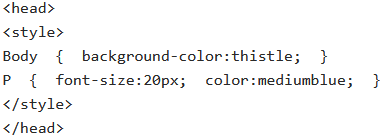
\includegraphics
	{../LaTeX/Images/css_internal.PNG}
	\caption{Modul intern de legare a codului CSS}
	\label{fig:311}
\end{figure}

Extern înseamnă scrierea codului într-un fișier separat salvat cu extensia ”.css”. Legătura dintre pagina web și regulile de stilizare din fișier se creează folosind elementul ”<link>”, după cum se poate observa în (Fig. \ref{fig:312}).

\begin{figure}[!htb]
	\centering
	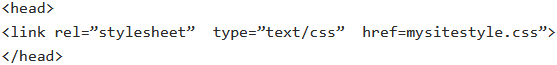
\includegraphics
	{../LaTeX/Images/css_external.PNG}
	\caption{Modul extern de legare a codului CSS}
	\label{fig:312}
\end{figure}

Codul ”inline” este codul CSS scris înăuntrul elementelor HTML, folosind proprietatea ”style”, reprezentat în (Fig. \ref{fig:313}).

\begin{figure}[!htb]
	\centering
	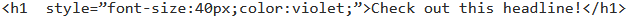
\includegraphics
	{../LaTeX/Images/css_inline.PNG}
	\caption{Modul inline de legare a codului CSS}
	\label{fig:313}
\end{figure}

Se preferă scrierea regulilor de stilizare într-un fișier separat deoarece astfel rezultă o separare între structura paginii web, elementele HTML și aspectul acesteia, regulile CSS. Codul este mai ușor de citit, mai ușor de întreținut și actualizat și permite o detectare mai ușoară a erorilor.
\\ \\
SCSS vine de la Sassy CSS și este un limbaj de preprocesare al cărui rezultat de compilare este cod CSS. În CSS este dificilă scrierea de reguli organizate și ușor de menținut deoarece lipsește suportul pentru cod imbricat (din engl. ”nested”), funcții și moștenire. Folosind SCSS se poate evita scrierea codului duplicat, prin construirea de bucăți de cod reutilizabile și se pot scrie secvențe de cod imbricate, care sunt structurate și ușor de citit (Fig. \ref{fig:314}).
\\ \\

\begin{figure}[!htb]
	\centering
	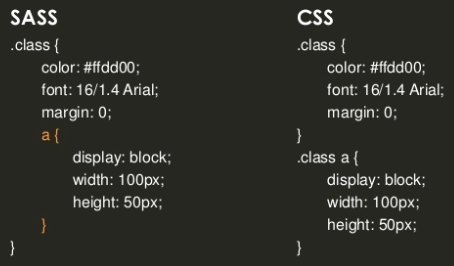
\includegraphics
	{../LaTeX/Images/scss_nesting.PNG}
	\caption{Secvență de cod ”nested”}
	\label{fig:314}
\end{figure}

Simbolul ”.” din ”.class” reprezintă o clasă de reguli de stilizare care se poate aplica unuia sau mai multor elemente HTML, spre deosebire de simbolul ”\#” care definește o regulă aplicabilă în mod unic unui singur element.
După cum se poate observa în (Fig. \ref{fig:314}), codul ”nested” evită dublarea selectorului ”.class” atunci când se face referire la elementul ”<a>”, de tip ancoră.
\\ \\
SCSS oferă suport pentru așa numitele ”directive de control”, care pot defini o regulă de stilizare dacă o anumită condiție este îndeplinită. Una dintre aceste directive este ”@if” care funcționează asemenea structurilor alternative din limbajele de programare precum C\#. Folosind ”@if”, se aplică unui element ”<div>” o margine albă de grosime de 1 pixel, dacă rezultatul condiției este egal cu 4, după cum este ilustrat în (Fig. \ref{fig:315}).

\begin{figure}[!htb]
	\centering
	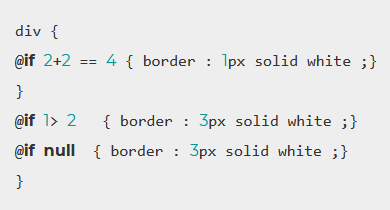
\includegraphics[width=0.4\textwidth]
	{../LaTeX/Images/scss_if-1.PNG}
	\caption{Directiva de control ”@if”}
	\label{fig:315}
\end{figure}

După evaluarea condiției din ”@if” și compilarea codului, rezultă regula de stilizare reprezentată în (Fig. \ref{fig:316}).

\begin{figure}[!htb]
	\centering
	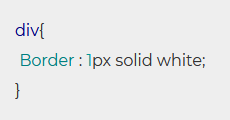
\includegraphics[width=0.2\textwidth]
	{../LaTeX/Images/scss_if-2.PNG}
	\caption{Directiva de control ”@if”}
	\label{fig:316}
\end{figure}
	
	\chapter{Framework-uri web}
	% !TeX root = ../FoodSpy.tex
% \section{Framework-uri web}

\section{Angular}
Numele ”Angular” vine de la caracterele ”<” și ”>” (în engleză, ”angled brackets”) care delimitează numele tuturor tag-urilor din HTML, de exemplu ”<a>” sau ”<div>”.
Angular este o platformă de dezvoltare, bazată pe limbajul TypeScript, care este un superset al limbajului JavaScript. Angular este un framework care face posibilă implementarea într-un mod trivial a cerințelor complexe ale aplicațiilor web, cum ar fi animații sau ”data binding”.
\\ \\
Platforma Angular oferă un mod de lucru bazat pe componente individuale care duce cu ușurință la construirea de aplicații web scalabile, dar și la posibilitatea reutilizării acestor componente în alte aplicații.
Angular vine integrat cu o multitudine de biblioteci care acoperă o gamă largă de cazuri de utilizare, printre care comunicarea cu un server și validarea formularelor HTML (Fig. \ref{fig:41}).

\begin{figure}[!htb]
	\centering
	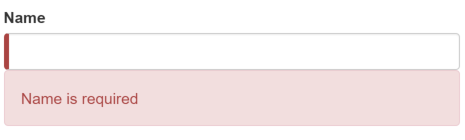
\includegraphics
	{../LaTeX/Images/angular_hero-form-2.PNG}
	\caption{Validarea câmpului ”Name” din formular}
	\label{fig:41}
\end{figure}

Mai mult, Angular este gândit să faciliteze actualizarea cât mai ușoară a aplicației, de aceea pune la dispoziție o suită de unelte care ajută la dezvoltarea, testarea și actualizarea codului printre care și ”Live Reload”, o funcționalitate prin care aplicația web este recompilată și deservită la orice modificare a codului-sursă.

\subsection{Components}
Asemenea blocurilor de LEGO, componentele Angular sunt puse laolaltă pentru a construi o aplicație web. O componentă (Fig. \ref{fig:42}) este formată dintr-o clasă TypeScript, adnotată cu decoratorul ”@Component”, un șablon HTML și opțiuni de stilizare.
\\ \\
În clasa TypeScript este scris codul care determină funcționalitatea componentei, șablonul HTML spune cum este structurată componenta, iar opțiunile de stilizare definesc aspectul acesteia. Această separare ajută la testarea mai ușoară a codului și lizibilitatea acestuia.

\begin{figure}[!htb]
	\centering
	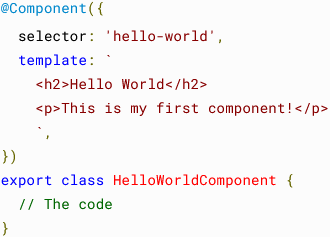
\includegraphics
	{../LaTeX/Images/angular_components.PNG}
	\caption{O componentă Angular}
	\label{fig:42}
\end{figure}

Componenta se folosește printr-un apel după numele descris sub proprietatea ”selector”, în cazul acesta ”<hello-world></hello-world>”.

\subsection{Templates}
”Template” sau ”șablonul” descrie felul în care este structurată componenta folosind limbaj HTML. Limbajul HTML poate fi scris ”inline”, cum se vede în (Fig. \ref{fig:42}) sub proprietatea ”template” sau poate fi scris într-un fișier separat cu extensia ”.html”.
Angular extinde capabilitățile limbajului HTML oferind așa numitele ”directives”, care sunt clase ce pot modifica în mod dinamic structura aplicației.
\\ \\
De exemplu, ”*ngIf” poate fi folosit pe un ”<div>” (dar și alte tag-uri HTML) pentru a-l afișa sau nu în funcție de valoarea unei variabile de tip ”boolean”, astfel:

\begin{verbatim}
	<div *ngIf=”showDiv”>
	<p> Dacă ”showDiv” este ”true” atunci ”<div>” este vizibil în pagină </p>
	</div>
	
	<div *ngIf=”!showDiv”>
	<p> Dacă ”showDiv” este ”false” atunci ”<div>” nu este vizibil în pagină </p>
	</div>
\end{verbatim}

De reținut este faptul că ”showDiv” este o variabilă ce a fost definită în clasa TypeScript a componentei.

\subsection{Dependency Injection}
Prin ”dependency injection” a se înțelege un design pattern prin care este posibilă scrierea de cod-sursă mai flexibil și mai ușor de testat. În Angular, prin ”dependency injection”, într-o clasă se pot declara dependințe către alte clase, fără să fie necesară instanțierea explicită a lor - instanțierea se efectuează în mod automat.
O clasă către care este definită o dependință din altă clasă trebuie să fie adnotată cu decoratorul ”@Injectable”, astfel:

\begin{figure}[!htb]
	\centering
	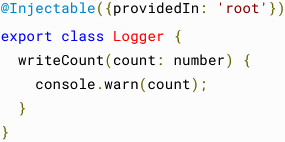
\includegraphics
	{../LaTeX/Images/angular_injectable.PNG}
	\caption{”Logger” este o clasă ce poate fi ”injectată”}
	\label{fig:44}
\end{figure}

Funcția ”writeCount()” din clasa ”Logger” este folosită mai departe în interiorul clasei ”HelloWorldDependencyInjectionComponent”, după cum se vede în (Fig. \ref{fig:45}).

\begin{figure}[!htb]
	\centering
	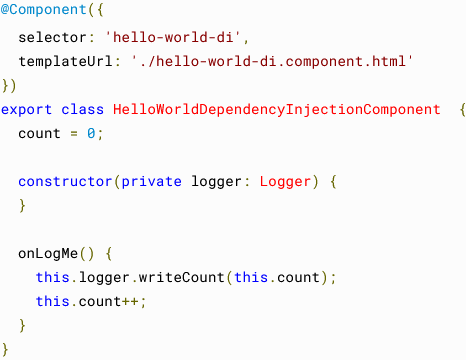
\includegraphics
	{../LaTeX/Images/angular_dependency-injection.PNG}
	\caption{”HelloWorldDependencyInjectionComponent” cu membrul ”private logger”}
	\label{fig:45}
\end{figure}

A se observa constructorul clasei ”HelloWorldDependencyInjectionComponent”, unde s-a definit o dependință către clasa ”Logger” prin membrul ”private logger”.

\section{ASP.NET Core}
ASP.NET Core este un framework web, care rulează pe platforma .NET și .NET Core. Bazat pe limbajul de programare C\#, ASP.NET Core suportă construirea serviciilor REST (așa numitele API-uri web).
Un ”request” sau o ”cerere” venită către un asemenea serviciu REST este tratată de către un controller. În ASP.NET Core, un controller este o clasă ce derivă din clasa de bază ”ControllerBase”.

\begin{figure}[!htb]
	\centering
	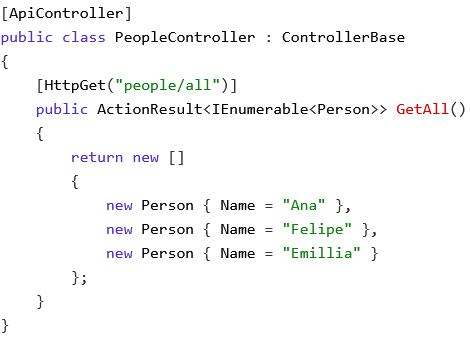
\includegraphics[width=0.8\textwidth]
	{../LaTeX/Images/asp_controller-1.PNG}
	\caption{”PeopleController” este un exemplu de controller}
	\label{fig:46}
\end{figure}

Deoarece ”PeopleController” este adnotat cu atributul ”[HttpGet("people/all")]”, acesta este capabil să răspundă cererilor metodei ”GET” efectuate la URL-ul ”/people/all”.
\\ \\
”people/all” se mai numește ”endpoint” și intrinsec este configurat să răspundă într-un mod serializabil, sub forma unui JSON, după cum se poate observa în (Fig. \ref{fig:47}).

\begin{figure}[!htb]
	\centering
	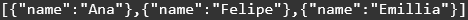
\includegraphics
	{../LaTeX/Images/asp_response.PNG}
	\caption{Exemplu de răspuns dat de un controller}
	\label{fig:47}
\end{figure}

După cum se poate observa și în exemplele de mai sus, ASP.NET Core permite definirea ”inline” a endpoint-urilor și metodelor REST prin adnotări, folosind atribute.
Un exemplu de controller capabil să răspundă la metodele ”GET” și ”POST” este ilustrat în (Fig. \ref{fig:48}).

\begin{figure}[!htb]
	\centering
	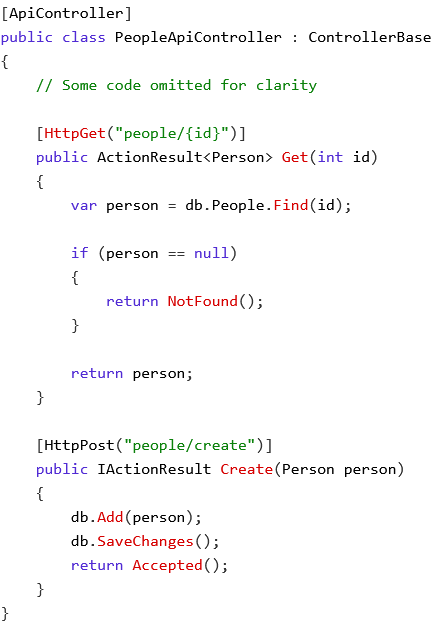
\includegraphics[width=0.8\textwidth]
	{../LaTeX/Images/asp_controller-2.PNG}
	\caption{Exemplu controller}
	\label{fig:48}
\end{figure}

În practică deci, un web API construit folosind ASP.NET Core nu este altceva decât o colecție de unul sau mai multe controller-e care sunt capabile să răspundă cererilor venite din partea interfeței-utilizator (și nu numai).
	
	\chapter{Tehnologii}
	% !TeX root = ../FoodSpy.tex
% \section{Tehnologii}

\section{MikroORM și ORM}
ORM sau Object-Relational Mapping este o tehnică de a interoga și manipula datele dintr-o bază de date folosind o paradigmă orientată pe obiect. MikroORM este o bibliotecă TypeScript care implementează această tehnică.
MikroORM încapsulează codul necesar manevrării datelor și astfel nu mai este nevoie de scrierea explicită a interogărilor.
\\ \\
Mai mult, biblioteca permite interacțiunea directă cu obiectele din baza de date folosind același limbaj în care este scris codul-sursă al aplicației - în cazul nostru, TypeScript.
\\ \\
MikroORM prezintă o serie de avantaje printre care faptul că utilizarea procedurilor stocate sau a tranzacțiilor se face la fel de simplu precum un apel de funcție, dar și faptul că modelul de date este definit o singură dată, ceea ce îl face ușor de actualizat și menținut. Un exemplu de model de date este ”User”. ”User” modelează utilizatorul aplicației, prin câmpuri precum ”email”, și este reprezentat în (Fig. \ref{fig:51}).

\begin{figure}[!htb]
	\centering
	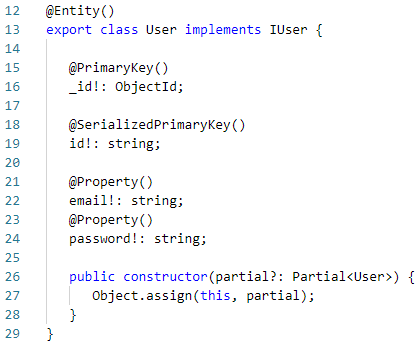
\includegraphics
	{../LaTeX/Images/mikroorm_user.PNG}
	\caption{Model de date MikroORM}
	\label{fig:51}
\end{figure}


\section{MongoDB și MongoDB Atlas}
MongoDB este un sistem de gestiune a bazelor de date orientat pe document. Deoarece un document este asemenea unui obiect JSON, câmpurile conținute în acesta pot să difere de la document la document și de asemenea, structura acestuia se poate modifica de-a lungul timpului. MongoDB permite o asociere directă între documentul din baza de date și obiectul din codul-sursă al aplicației, oferind programatorului posibilitatea de a manipula datele cu ușurință.

\begin{figure}[!htb]
	\centering
	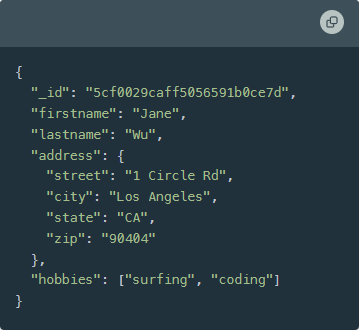
\includegraphics
	{../LaTeX/Images/mongodb_document.PNG}
	\caption{Document MongoDB}
	\label{fig:52}
\end{figure}

%maybe add \\ \\ here
La rădăcini, MongoDB este un sistem de gestiune scalabil și pretabil pentru a rula pe sisteme distribuite - aici intervine MongoDB Atlas care este serviciul MongoDB găzduit în cloud. Atlas pune la dispoziție toate funcționalitățile serviciului MongoDB, dar în același timp automatizează partea de administrare a bazei de date, de la configurarea acesteia până la efectuarea operației de ”backup”.
\\ \\
În oferta de găzduire în cloud există și un nivel gratis, așa numitul ”M0 Sandbox”, care poate fi folosit pentru acomodare cu serviciul MongoDB, pentru prototipare și pentru primele implementări ale bazei de date.


\section{Node.js}
Node.js este un mediu de rulare JavaScript construit pe engine-ul V8 din Chrome. Este folosit pentru a rula aplicații web în afara browser-ului clientului. Deoarece folosește un mediu de rulare asincron, bazat pe evenimente, Node.js este gândit pentru scalabilitatea aplicațiilor de rețea, fiind capabil să administreze un număr mare de conexiuni în mod concurent.
\\ \\
Un modul Node.js este asemenea unei librării JavaScript care poate fi inclus înăuntrul unei aplicații pentru a facilita anumite funcționalități. De exemplu, în (Fig. \ref{fig:53}) este ilustrată utilizarea modului HTTP care face posibil crearea unui server web, care ascultă pe portul 2000.

\begin{figure}[!htb]
	\centering
	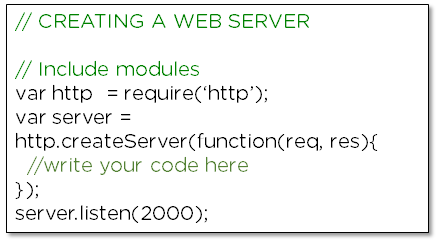
\includegraphics[width=0.6\textwidth]
	{../LaTeX/Images/nodejs_http.PNG}
	\caption{Modulul HTTP din Node.js}
	\label{fig:53}
\end{figure}

Față de mediul de rulare convențional, bazat pe thread-uri, Node.js are avantajul că funcțiile nu execută operații de input / output, deci procesul de rulare al aplicației nu este blocat niciodată. Mai mult, librăria Express din Node.js poate fi utilizată în diferite scenarii, de la aplicații de chat în timp real până la API-uri REST.


\section{Express}
Node.js nu oferă suport pentru diferitele verbe HTTP, precum GET, POST sau DELETE. De asemenea, nu poate servi fișiere statice și nici nu poate trata cererile care pot veni la diferite URL-uri, așa numitele ”rute” sau ”endpoint”-uri. Pentru aceste cazuri, este necesară implementarea manuală sau folosirea unui framework web, în speță, Express.
\\ \\
Express adresează neajunsurile Node.js enumerate mai sus prin pachete ”middleware” și mai mult decât atât, aceste pachete pot fi folosite pentru lucrul cu sesiuni sau cookie-uri, extragerea parametrilor din URL sau a datelor transmise prin corpul cererilor POST.

\begin{figure}[!htb]
	\centering
	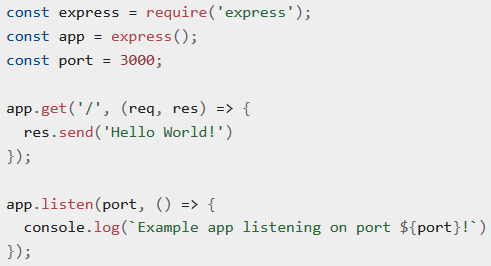
\includegraphics
	{../LaTeX/Images/express_hello.PNG}
	\caption{”Hello World” în Express}
	\label{fig:54}
\end{figure}

%maybe add \\ \\ here
Inițial, se importă modulul Express prin ”require(‘express’)”. Aplicația Express se instanțiază prin ”const app = express()”. Cu ajutorul ”app” definim ”endpoint”-urile tratate de API. În cazul prezentat în (Fig. \ref{fig:54}), ”app.get()” definește o funcție care va fi apelată atunci când se face un request GET la URL-ul rădăcină, adică ”/”. Răspunsul se trimite înapoi folosind ”send()” și va întoarce string-ul ”Hello World”. Cu ”app.listen()” se pornește server-ul care ascultă pe portul 3000 și care poate fi accesat la adresa ”localhost:3000”.


\section{NPM și publicarea pachetului ”FoodSpy-shared”}
NPM este manager-ul de pachete pentru Node.js. A fost creat în 2009 ca un proiect care să ajute dezvoltatorii JavaScript să partajeze cu ușurință secvențe de cod sub formă de module [REF](referință către Node.js) ambalate ca pachete. Registrul NPM este o colecție publică de astfel de pachete care sunt folosite de către comunitatea JavaScript pentru dezvoltarea aplicațiilor web sau aplicațiilor mobile. NPM pune la dispoziție un client care poate fi folosit în linie de comandă și oferă dezvoltatorilor capabilitatea de a instala, folosi și de a publica propriile pachete.
\\ \\
”FoodSpy-shared” este un pachet propriu, disponibil în registrul public NPM. Acesta conține o colecție de constante, interfețe și enum-uri folosite în aplicația Angular, dar și în API-ul care administrează datele despre utilizatori. Una dintre aceste interfețe este ”IUser”, ilustrată în (Fig. \ref{fig:55}). ”IUser” definește contractul care trebuie îndeplinit atât pe partea de front-end cât și pe partea de back-end, când vine vorba de manipularea datelor despre un utilizator. Adăugarea pachetului ”FoodSpy-shared” și implementarea interfeței ”IUser” în API este ilustrată în (Fig. \ref{fig:56}).

\begin{figure}[!htb]
	\centering
	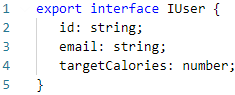
\includegraphics
	{../LaTeX/Images/npm_iuser.PNG}
	\caption{Interfața ”IUser”}
	\label{fig:55}
\end{figure}

\begin{figure}[!htb]
	\centering
	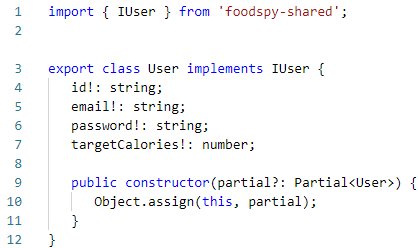
\includegraphics
	{../LaTeX/Images/npm_user.PNG}
	\caption{Implementarea interfeței ”IUser” în API}
	\label{fig:56}
\end{figure}


\section{Heroku}
Heroku este o platformă care pune la dispoziție posibilitatea de a construi, implementa și rula aplicații găzduite în cloud. Spre deosebire de Amazon Web Services sau Windows Azure, care oferă doar infrastructura în cloud necesară pentru a găzdui aplicația, Heroku oferă un serviciu de management asupra infrastructurii, care abstractizează toate detaliile legate de configurare și implementare. Astfel, Heroku permite dezvoltatorilor să concentreze toate resursele spre implementarea aplicației.
Heroku suportă o colecție de limbaje de programare și framework-uri, printre care JavaScript și Node.js.
\\ \\
Platforma pune la dispoziție toate uneltele necesare implementării unei aplicații, inclusiv administrarea mediului de rulare a aplicației și administrarea laturii DevOps. Din acest motiv, Heroku este un loc potrivit pentru a învăța despre microservicii și metodologii de implementare, precum livrarea continuă (”continuous delivery”). Mai mult decât atât, oferă un abonament destinat exclusiv studenților care permite utilizarea platformei pentru o perioadă de doi ani, suficient timp pentru a exersa orice limbaj de programare și orice șablon arhitectural.


\section{Utilitare (Postman, Git și GitHub)}
Postman este un utilitar interactiv prin care se pot examina endpoint-urile unui API. Postman poate fi folosit pe tot parcursul dezvoltării unei aplicații deoarece dispune de o interfață grafică care permite construirea și trimiterea de request-uri HTTP. De asemenea, se poate folosi pentru citirea și validarea răspunsurilor oferite de către API. Un exemplu de request trimis direct din Postman către ”FoodSpyAPI”, care interoghează baza de date pentru alimente care au în componența numelui termenul ”magiun” este reprezentat în (Fig. \ref{fig:57}).

\begin{figure}[!htb]
	\centering
	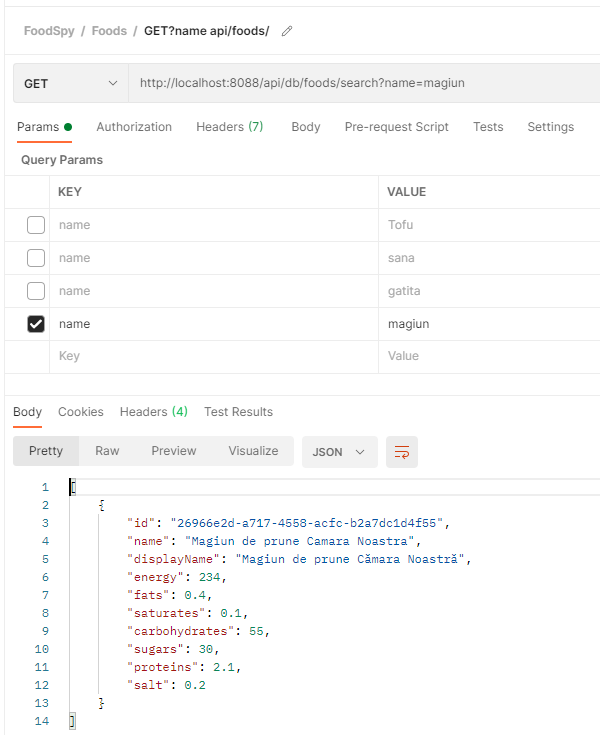
\includegraphics[width=0.8\textwidth]
	{../LaTeX/Images/postman_magiun.PNG}
	\caption{Request ”GET” trimis din Postman}
	\label{fig:57}
\end{figure}

%maybe add \\ \\ here
Git este un sistem de versionare distribuit care poate urmări schimbări în fișiere. Git este folosit de programatori pentru a colabora la scrierea codului-sursă în procesul de dezvoltare software. A fost creat în anul 2005 și a fost gândit pentru a fi eficient, pentru a păstra integritatea datelor și pentru a oferi suport pentru numeroase medii de dezvoltare.
\\ \\
Git urmărește schimbările în fișier pe toată durata dezvoltării software, ceea ce înseamnă că în orice moment, codul-sursă poate fi revizuit sau poate fi adus la o versiune precedentă.
\\ \\
Git se instalează și rulează pe sistemul local și nu are nevoie de conexiune la internet pentru a funcționa. Față de alte sisteme de versionare, Git este ușor de folosit și gratis și a fost gândit să lucreze în principal cu fișiere text, adică exact tipul de fișiere folosit pentru a salva cod-sursă. Întregul cod-sursă este menținut sub evidența sistemului de versionare într-un director care poartă numele de ”repository”. Avantajul major al Git este așa numitul ”branching model”. Prin procesul de ”branching” se pot crea ”ramuri”, care sunt copii independente ale repository-ului. Asta se traduce prin ușurința de a testa și implementa noi funcționalități în aplicație, fără a afecta munca celorlalți participanți la dezvoltarea aplicației.
\\ \\
GitHub este un serviciu de găzduire a unui repository. Este bazat exclusiv pe infrastructură cloud și este o bază de date care reține o colecție de repository-uri. GitHub este practic o versiune online a unui repository local și astfel oferă posibilitatea de a partaja un repository sau de a adăuga alți programatori care pot contribui în mod independent la dezvoltarea aplicației. Cu alte cuvinte, GitHub extinde funcționalitățile oferite de Git printr-o interfață intuitivă și unelte de management asupra unui repository. Un instantaneu al repository-ului care conține codul-sursă al aplicației ”FoodSpy” este reprezentat în (Fig. \ref{fig:58}). Se poate observa că branch-ul ”calculate-calories” a suferit 9 modificări de la momentul în care a fost clonat din branch-ul principal, adică ”master”.

\begin{figure}[!htb]
	\centering
	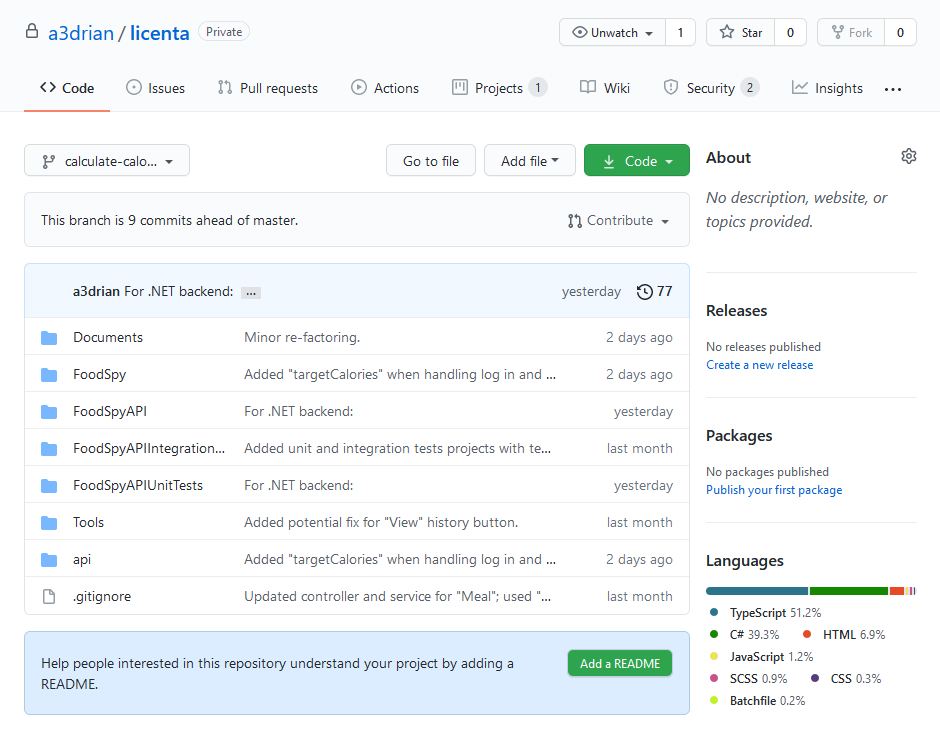
\includegraphics[width=0.9\textwidth]
	{../LaTeX/Images/github_repo.PNG}
	\caption{Repository-ul ”FoodSpy”}
	\label{fig:58}
\end{figure}
	
	\chapter{Descrierea aplicației}
	% !TeX root = ../FoodSpy.tex
% \section{Descrierea aplicației}

\begin{figure}[!htb]
	\centering
	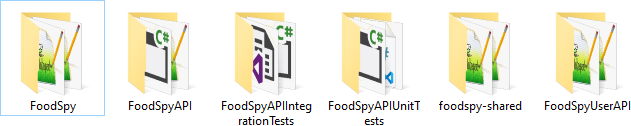
\includegraphics[width=0.8\textwidth]
	{../LaTeX/Images/implementare_arhitectura.PNG}
	\caption{Arhitectura aplicației FoodSpy}
	\label{fig:61}
\end{figure}

Arhitectura aplicației FoodSpy presupune o implementare realizată pe mai multe nivele de infrastructură, nivele ce sunt detaliate în rândurile următoare.
\\ \\
Proiectul ”FoodSpy” reprezintă nivelul clientului sau nivelul de prezentare, adică interfața grafică prin care utilizatorul interacționează cu aplicația.
\\ \\
”FoodSpyUserAPI” este interfața de programare care efectuează comunicarea cu server-ul care se ocupă de administrarea utilizatorilor și a datelor acestora.
\\ \\
Proiectul care se ocupă de persistența datelor reținute în jurnalul fiecărui utilizator este ”FoodSpyAPI”. Acesta este responsabil pentru stocarea informațiilor legate de mâncărurile pe care utilizatorii le pot folosi pentru a-și compune mesele și pentru a înregistra aportul caloric în jurnal.
\\ \\
Nivelul de testare este acoperit de proiectele ”FoodSpyAPIIntegrationTests” și ”FoodSpyAPIUnitTests”.
\\ \\
”foodspy-shared” este proiectul care reprezintă nivelul auxiliar, un nivel care face posibilă partajarea dependințelor aplicației. Acesta conține o colecție de enumerări și interfețe care sunt folosite atât la nivelul clientului cât și la nivelul interfețelor de programare (API-urilor).

\section{Clientul}
Nivelul clientului este împărțit pe mai multe componente Angular.
\\ \\
”Auth” constituie componenta care administrează pagina de autentificare în aplicație. La baza acestei componente este un formular HTML. Pentru un utilizator care urmează să își creeze un cont, formularul are 3 câmpuri: e-mail-ul, parola și aportul zilnic de calorii pe care acesta dorește să-l atingă în fiecare zi. Pentru e-mail se folosește o validare bazată pe o expresie regulată care impune în componența sa existența unui domeniu (”.com”, ”.ro”, etc.). Parola trebuie să aibă un număr minim de caractere, număr definit de o constantă, iar aportul este exprimat ca un număr întreg cuprins într-un anumit interval.
\\ \\
Pentru cazul în care utilizatorul are deja cont și efectuează operația de autentificare în aplicație, formularul nu mai afișează câmpul numărului de calorii.
Se observă astfel faptul că același formular este folosit pentru procesul de înregistrare, dar și pentru procesul de autentificare. Această implementare este posibilă folosind directiva ”*ngIf”.

\begin{figure}[!htb]
	\centering
	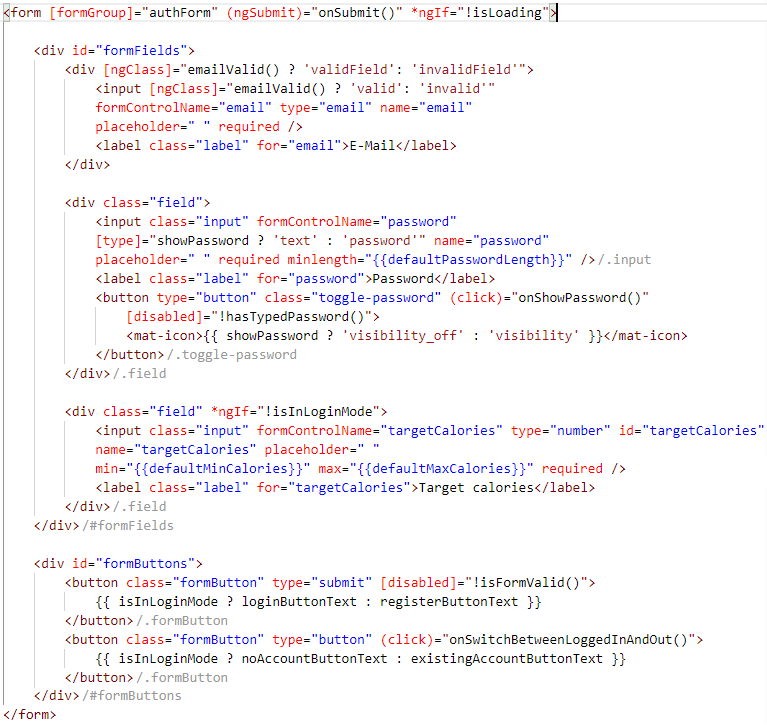
\includegraphics[width=0.95\textwidth]
	{../LaTeX/Images/implementare_form.PNG}
	\caption{Formularul de înregistrare și autentificare în aplicație}
	\label{fig:62}
\end{figure}

”Auth” utilizează serviciul de autentificare ”AuthService”. Acesta validează datele introduse în formular și trimite un request ”POST” către interfața de programare care se ocupă de administrarea utilizatorilor. Request-ul ”POST” este împachetat într-o interfață ”IAuthResponseData” compusă din proprietățile ”email”, ”password” și ”targetCalories”. Interfața este partajată cu ”FoodSpyUserAPI” pentru a facilita despachetarea cu ușurință a informațiilor conținute în request-ul ”POST”.

\begin{figure}[!htb]
	\centering
	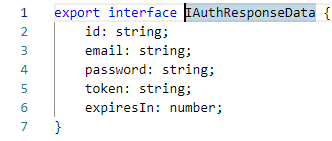
\includegraphics
	{../LaTeX/Images/implementare_iauthresponsedata.PNG}
	\caption{Interfața ”IAuthResponseData”}
	\label{fig:63}
\end{figure}

După înregistrare sau autentificare, utilizatorul este redirecționat către componenta ”Intakes”. ”Intakes” reprezintă tabloul de bord al aplicației și afișează numărul de calorii pe care acesta și le-a setat ca obiectiv de atins la momentul înregistrării.
De asemenea, oferă posibilitatea de a urmări istoricul utilizării aplicației, pe zile, ordonate de le cea mai îndepărtată zi, la cea mai apropiată. Acest istoric reprezintă de fapt jurnalul aportului de calorii al utilizatorului.

\begin{figure}[!htb]
	\centering
	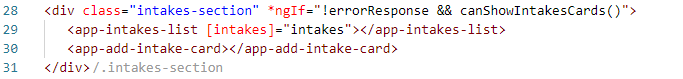
\includegraphics[width=0.9\textwidth]
	{../LaTeX/Images/implementare_intakes.PNG}
	\caption{Componenta ”Intakes”}
	\label{fig:64}
\end{figure}

Obiectul ”intakes” de la linia 29 din (Fig. \ref{fig:64}) este populat cu rezultatul unui request ”POST” către ”FoodSpyAPI” care întoarce o listă de intrări din jurnalul unui anume utilizator, identificat prin adresa acestuia de e-mail. 
Nu se face un request ”GET” deoarece acest endpoint din (Fig. \ref{fig:65}) permite sortarea intrărilor din jurnal, din punct de vedere cronologic, dacă se populează o proprietate numită ”sortOrder” cu valoarea 0 pentru ascendent sau cu valoarea 1 pentru descendent.

\begin{figure}[!htb]
	\centering
	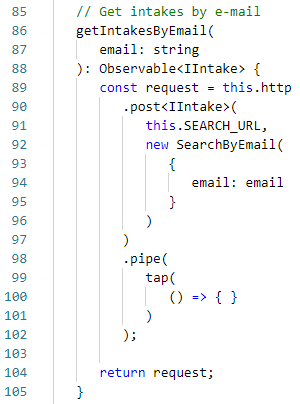
\includegraphics[width=0.6\textwidth]
	{../LaTeX/Images/implementare_getintakesbyemail.PNG}
	\caption{Request ”POST” către ”/api/db/intakes/search/”}
	\label{fig:65}
\end{figure}

În tabloul de bord, fiecare dintre aceste zile care face parte din istoric sunt conținute într-o componentă numită ”IntakeCard”. În ”IntakeCard”, istoricul nu este detaliat, afișează doar procentul de completare al aportului de calorii, și cantitatea totală de grăsimi, carbohidrați și zaharuri pe care utilizatorul le-a consumat în ziua respectivă.
\\ \\
Detaliile precum mâncărurile care fac parte din componența unei mese și cantitatea fiecăruia dintre mâncăruri consumate de utilizator sunt afișate în componenta ”IntakeHistory”, la care se ajunge prin intermediul unui hyperlink. Hyperlink-ul este atașat unei element ”<h2>” prin evenimentul ”(click)”, după cum se poate observa în (Fig. \ref{fig:66}). Elementul ”<h2>” exprimă numărul de mese consumate de utilizator într-o anumită zi.

\begin{figure}[!htb]
	\centering
	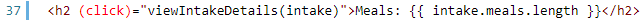
\includegraphics[width=0.95\textwidth]
	{../LaTeX/Images/implementare_hyperlink.PNG}
	\caption{Hyperlink atașat pe evenimentul ”(click)”}
	\label{fig:66}
\end{figure}

”Intakes” face legătură către ”AddMeal” prin componenta ”AddIntakeCard”. Cu ajutorul ”AddMeal”, un utilizator poate căuta mâncărurile pe care să la adauge la o masă, iar masa o poate adăuga la jurnalul din ziua respectivă.
\\ \\
”AddMeal” este cea mai complicată dintre componente, deoarece ea implementează funcționalitatea pentru căutarea mâncărurilor în baza de date și construcția unui obiect de tip ”IIntake”, care reprezintă o zi din jurnal.
\\ \\
Când utilizatorul accesează componenta ”AddMeal”, se inițializează obiectul de tip ”IIntake” cu valori default. De exemplu, o proprietate a acestui obiect este ”createdAt”, care va reține momentul la care s-a adăugat în jurnal prima masă. Se mai inițializează proprietatea ”email” cu e-mail-ul utilizatorului și ”targetCalories” cu obiectivul setat de utilizator.

\begin{figure}[!htb]
	\centering
	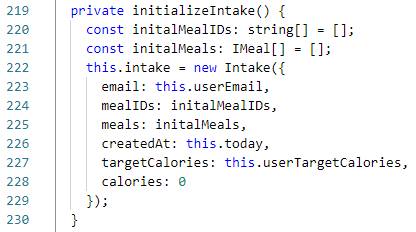
\includegraphics[width=0.8\textwidth]
	{../LaTeX/Images/implementare_initializeintake.PNG}
	\caption{Inițializarea componentei ”Intakes”}
	\label{fig:67}
\end{figure}

Căutarea mâncărurilor din baza de date se face folosind un ”<input>” de tip ”text” atașat la o funcție care preia termenul de căutare introdus de către utilizator și face un request ”GET” către ”FoodsService”. Termenul de căutare populează parametrul din URL numit ”name” și asta va determina endpoint-ul definit în ”FoodSpyAPI” să returneze o listă de mâncăruri filtrate după nume. Un exemplu de request ”GET” după criteriul numelui este ”/api/db/foods/search?name=ciocolata”.

\begin{figure}[!htb]
	\centering
	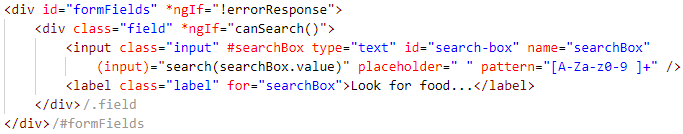
\includegraphics[width=0.9\textwidth]
	{../LaTeX/Images/implementare_search.PNG}
	\caption{Bara de căutare a mâncărurilor după nume}
	\label{fig:68}
\end{figure}

Odată găsită mâncarea în baza de date, utilizatorul poate deschide o căsuță de dialog, care reprezintă componenta ”EditFoodDialogue”. Aici, utilizatorul poate vedea mai multe detalii despre mâncarea selectată în urma căutării, printre care cantitatea de săruri sau proteine și de asemenea poate introduce cantitatea de mâncare, exprimată în grame.
\\ \\
Pentru cantitate este construită o validare care impune valoarea acesteia să nu poată depăși 1000 de grame. Validarea este ilustrată în (Fig. \ref{fig:69}). Aceasta poartă numele de ”foodQuantityValidator” și este implementată folosind clasa abstractă ”AbstractControl”. ”AbstractControl” permite accesul la valoarea introdusă de utilizator în formular și astfel se pot impune restricții asupra acesteia.

\begin{figure}[!htb]
	\centering
	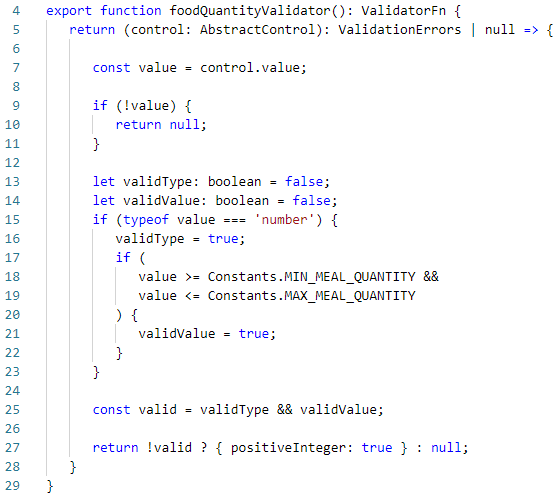
\includegraphics[width=0.9\textwidth]
	{../LaTeX/Images/implementare_foodqtyvalidator.PNG}
	\caption{Validarea pentru cantitatea de mâncare}
	\label{fig:69}
\end{figure}

După adăugarea unei mâncăruri, utilizatorul poate selecta tipul de masă pe care acesta a consumat-o. Tipurile de masă sunt ”Breakfast”, ”Lunch”, ”Dinner” sau ”Snack”. La momentul alegerii unuia dintre tipuri, formularul este valid și utilizatorului i se permite să înregistreze masa în jurnal.
\\ \\
Când se înregistrează o masă, există două scenarii.
\\ \\
Primul scenariu este acela în care utilizatorul nu are nicio intrare în jurnalul zilei respective, iar al doilea scenariu reprezintă modificarea unui jurnal deja existent.
În primul scenariu, implementarea este simplă deoarece este suficient să adăugăm masa în colecția ”Meals” din baza de date și apoi să introducem ID-ul acestei mese în proprietatea ”mealIDs” a obiectului de tip ”IIntake”. Ultimul pas este să trimitem un request ”POST” către ”FoodSpyAPI” pentru a înregistra jurnalul în colecția ”Intakes” din baza de date.
\\ \\
Al doilea scenariu este mai complicat deoarece în primul rând trebuie să determinăm dacă această masă nou adăugată face parte dintr-un tip de masă care există deja în în obiectul ”IIntake”.
Dacă nu face parte, se persistă o masă nouă și se aduce referința în proprietatea ”mealIDs” prin ID, iar în final se execută un request ”PUT” pentru a modifica un ”Intake” deja existent. Dacă face parte, atunci trebuie identificată colecția de mese care are același tip cu tipul mesei pe care utilizatorul dorește să o adauge. După identificarea acesteia, se concatenează colecția existentă cu masa ce urmează să fie adăugată, se aduce referința (ID-ul) în obiectul ”IIntake” și din nou se modifică jurnalul (obiectul de tip ”IIntake”) prin același request ”PUT”.
\\ \\
După executarea oricăruia dintre cele 2 scenarii descrise mai sus, se reîncarcă pagina pentru a reflecta modificarea din obiectul ”IIntake”.

\begin{figure}[!htb]
	\centering
	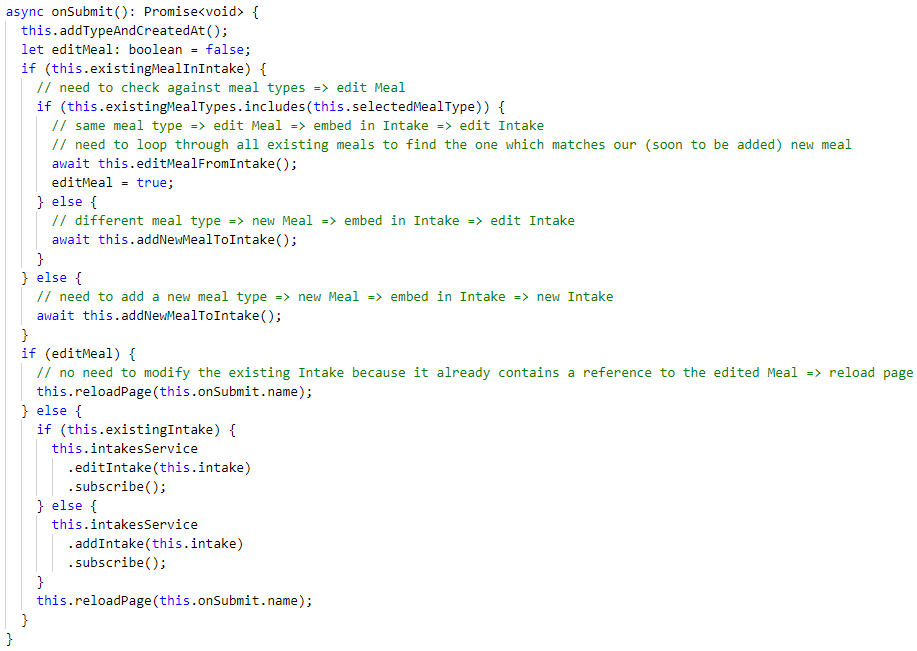
\includegraphics[width=0.95\textwidth]
	{../LaTeX/Images/implementare_addmeal.PNG}
	\caption{Adăugarea unei intrări în jurnalul zilnic}
	\label{fig:610}
\end{figure}

Prezent deasupra tuturor celorlalte componente, ”Header” (Fig. \ref{fig:611}) reprezintă antetul aplicației. Acesta afișează e-mail-ul utilizatorului autentificat, logo-ul aplicației și un buton pe care utilizatorul îl poate folosi pentru deconectare și redirecționare la componenta ”Auth”.

\begin{figure}[!htb]
	\centering
	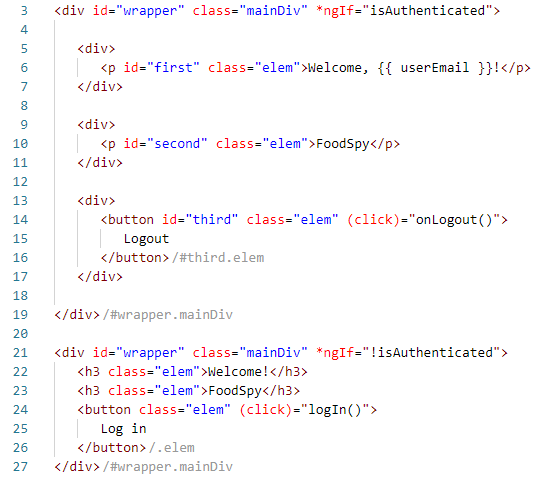
\includegraphics[width=0.8\textwidth]
	{../LaTeX/Images/implementare_header.PNG}
	\caption{Componenta ”Header”}
	\label{fig:611}
\end{figure}


\section{API pentru administrarea utilizatorilor}
Interfața de programare pentru administrarea utilizatorilor pune la dispoziție două endpoint-uri, un endpoint pentru operația de înregistrare a unui nou utilizator și unul pentru procesul de autentificare în aplicație.
\\ \\
La baza API-ului stă MikroORM, biblioteca TypeScript care implementează tehnica de a interoga și manipula datele dintr-o bază de date folosind o paradigmă orientată pe obiect. Cu ajutorul MikroORM, se definește o entitate care modelează profilul unui utilizator, dar și un manager peste această entitate care permite înregistrarea sau autentificarea acestuia în aplicație.
\\ \\
Pentru înregistrarea unui utilizator este nevoie să definim un endpoint pentru verbul ”POST” cu ajutorul unei rute. Din (Fig. \ref{fig:612}), se poate observa că ruta folosită pentru procesul de înregistrare este ruta rădăcină, adică ”/api/auth/register”.

\begin{figure}[!htb]
	\centering
	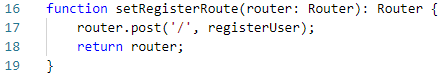
\includegraphics
	{../LaTeX/Images/userapi_rutaregister.PNG}
	\caption{Ruta pentru înregistrare}
	\label{fig:612}
\end{figure}

”registerUser” este funcția care face un apel către ”getUserByEmail” din ”UserService”. Funcția respectivă întoarce imediat o eroare dacă din corpul request-ului ”POST” lipsește e-mail-ul utilizatorului. Altfel, folosind manager-ul peste entități oferit de MikroORM, se caută utilizatorul identificat de e-mail-ul introdus în formularul din componenta ”Auth” din client. Dacă se găsește utilizatorul, detaliile despre acesta se returnează într-un obiect ”User”, iar dacă nu există, funcția întoarce ”null”.
\\ \\
În (Fig. \ref{fig:613}) este ilustrată funcția ”getUserByEmail”.

\begin{figure}[!htb]
	\centering
	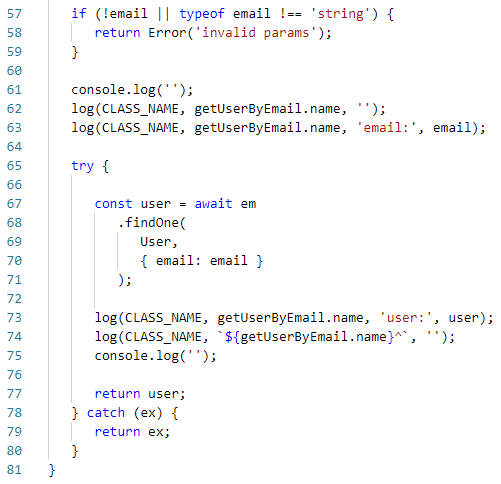
\includegraphics[width=0.9\textwidth]
	{../LaTeX/Images/userapi_getuserbyemail.PNG}
	\caption{Funcția ”getUserByEmail”}
	\label{fig:613}
\end{figure}

La momentul înregistrării, este important ca ”getUserByEmail” să returneze ”null”. Dacă returnează ”null”, înseamnă că utilizatorul nu există în baza de date și se poate înregistra cu succes folosind e-mail-ul, parola și obiectul caloric propus. Parola este criptată folosind biblioteca ”bcrypt” pentru a nu fi persistată în baza de date în format ”plain text”.
\\ \\
Dacă ”getUserByEmail” nu returnează ”null”, înseamnă că utilizatorului trebuie să îi fie afișat un mesaj de eroare care să-l atenționeze că există deja un cont creat cu același e-mail.

\begin{figure}[!htb]
	\centering
	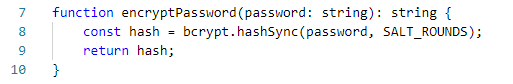
\includegraphics
	{../LaTeX/Images/userapi_bcrypt.PNG}
	\caption{Criptarea parolei folosind ”bcrypt”}
	\label{fig:614}
\end{figure}

Pentru autentificarea unui utilizator este nevoie să definim un endpoint pentru verbul ”POST” cu ajutorul unei rute. Din (Fig. \ref{fig:615}), se poate observa că ruta folosită pentru procesul de autentificare este ruta rădăcină, adică ”/api/auth/login”.

\begin{figure}[!htb]
	\centering
	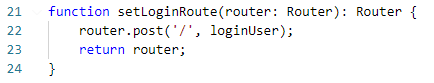
\includegraphics
	{../LaTeX/Images/userapi_rutalogin.PNG}
	\caption{Ruta pentru autentificare}
	\label{fig:615}
\end{figure}

Asemenea funcției ”registerUser”, funcția ”loginUser” face un apel către ”getUserByEmail” din ”UserService”.
\\ \\
La momentul autentificării, această funcție trebuie să returneze un obiect ”User”, care conține datele despre utilizator. În caz contrar, există scenariul în care utilizatorul nu există și trebuie mai întâi să se înregistreze sau există scenariul în care utilizatorul se află în baza de date. În acest caz, parola introdusă în formular este comparată cu parola persistată, iar dacă nu există o potrivire, un mesaj de eroare este afișat în client.

\begin{figure}[!htb]
	\centering
	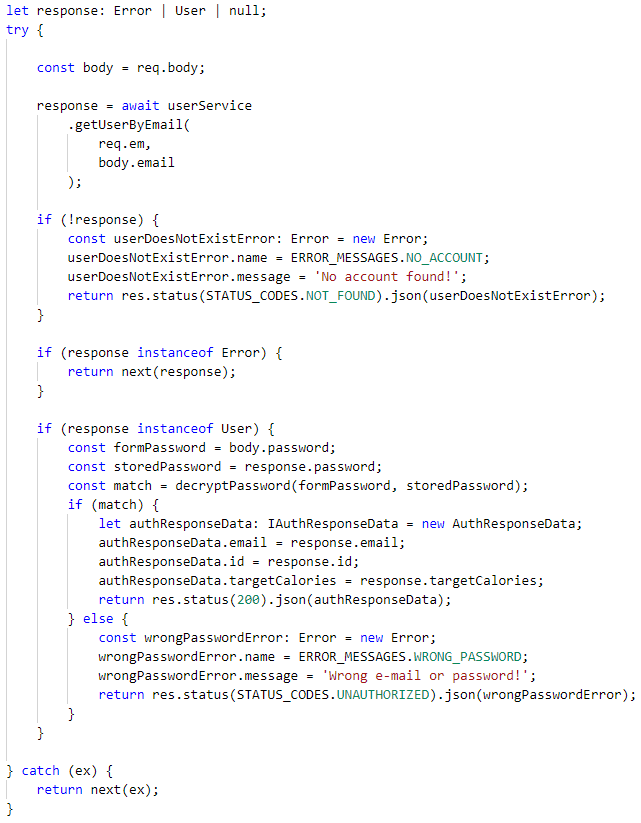
\includegraphics[width=0.9\textwidth]
	{../LaTeX/Images/userapi_loginuser.PNG}
	\caption{Corpul funcției ”loginUser”}
	\label{fig:616}
\end{figure}

La momentul pornirii server-ului care administrează datele despre utilizator, se caută un fișier numit ”.env” care conține string-ul de conectare la baza de date MongoDB precum și portul la care ascultă pentru cererile venite din partea clientului. ”.env” este interpretat de către API, care identifică string-ul de conectare și deschide portul de comunicare pentru client.
\\ \\
Fișierul ”.env” nu este înregistrat în repository-ul aplicației deoarece conține informații sensibile.


\section{API pentru gestiunea jurnalelor utilizatorilor}
Structura proiectului ”FoodSpyAPI” este reprezentată în (Fig. \ref{fig:616}).

\begin{figure}[!htb]
	\centering
	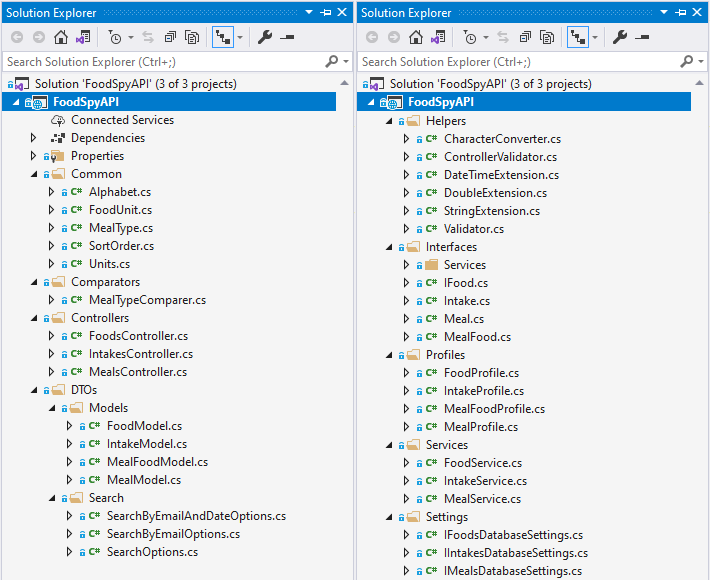
\includegraphics[width=0.8\textwidth]
	{../LaTeX/Images/fsapi_structura.PNG}
	\caption{Arhitectura proiectului ”FoodSpyAPI”}
	\label{fig:617}
\end{figure}

Directorul ”Common” conține clase și enumerări, precum ”Alphabet” sau ”MealType”. În ”Alphabet” există totalitatea caracterelor permise în aplicație, o reuniune a caracterelor alfabetului englez împreună cu literele cu diacritice din alfabetul limbii române. ”Alphabet” conține și o funcție ”ConvertDiacritic” care este utilizată pentru a îndepărta diacriticile dintr-un caracter.
\\ \\
”MealType” este o clasă statică care are în componența sa enumerarea ”MealType” folosită pentru definirea tipurilor de masă permise în aplicație. De asemenea, ”MealType” definește funcția ”GetMealTypesOrder” care are ca parametru de retur un ”Dictionary<string, uint>”. Dicționarul are ca utilitate sortarea meselor în funcție de tipul acestora, ”Breakfast” primul, ”Lunch” al doilea, ”Dinner” al treilea și ”Snack” ultimul.

\begin{figure}[!htb]
	\centering
	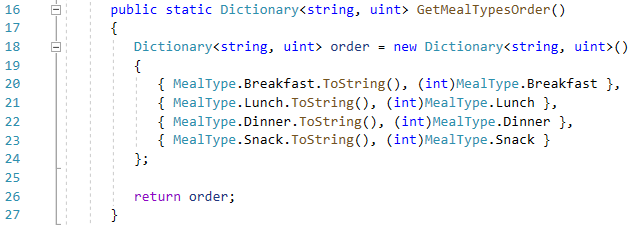
\includegraphics[width=0.8\textwidth]
	{../LaTeX/Images/fsapi_mealtype.PNG}
	\caption{Corpul funcției ”GetMealTypesOrder”}
	\label{fig:618}
\end{figure}

Dicționarul este folosit în funcția ”Compare” a clasei ”MealTypeComparer” din directorul ”Comparators”. În funcție de ponderea tipului de masă, clasa poate sorta mesele dintr-un jurnal în ordine crescătoare sau descrescătoare.

\begin{figure}[!htb]
	\centering
	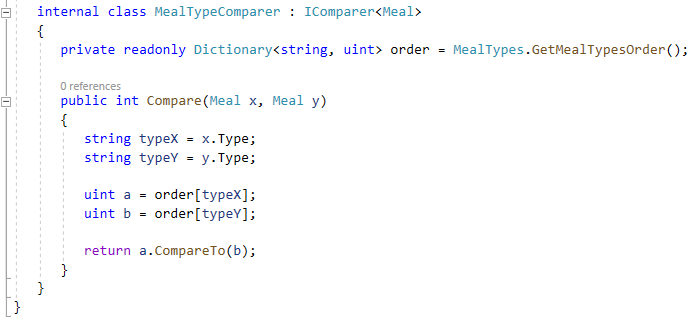
\includegraphics[width=0.8\textwidth]
	{../LaTeX/Images/fsapi_mealtypecomparer.PNG}
	\caption{Implementarea comparării tipurilor de mese}
	\label{fig:619}
\end{figure}

Interfața de programare pentru gestiunea jurnalelor utilizatorilor este compus din trei controller-e, ”IntakesController”, ”MealsController” și ”FoodsController”, din directorul ”Controllers”. Fiecare dintre acestea trei are definite endpoint-uri pentru verbele ”GET”, ”GET” cu parametrul din URL ”id”, ”POST”, ”PUT” și ”DELETE”.
\\ \\
”GET” returnează lista tuturor obiectelor de același tip cu tipul reprezentat de controller (”Intake”, ”Meal” sau ”Food”). ”GET” returnează un singur obiect identificat de parametrul ”id” din URL. ”POST” este folosit pentru adăugarea unui nou obiect, ”PUT” pentru editarea unui obiect deja existent, iar ”DELETE” pentru ștergerea unui obiect din baza de date.
\\ \\
Pentru implementarea anumitor endpoint-uri este nevoie mai mult de unul din aceste verbe. Spre exemplu, pentru ”PUT” trebuie mai întâi să inițiem un request ”GET” după parametrul ”id” din URL. Rezultatul acestui request va fi un obiect care ulterior poate fi modificat cu ajutorul request-ului ”PUT”.
\\ \\
Utilizatorul poate filtra mâncărurile din baza de date după criteriul numelui. De această filtrare se ocupă ”FoodsController” și funcția ”SearchFoodsByName”, ilustrată în (Fig. \ref{fig:620}). Această funcție primește ca parametru un obiect de tip ”string” care reprezintă termenul de căutare primit de la client. Cu ajutorul acestei funcții, a verbului ”GET” și a rutei ”/api/db/foods/search” se definește endpoint-ul care filtrează mâncărurile.

\begin{figure}[!htb]
	\centering
	\includegraphics[width=0.9\textwidth]
	{../LaTeX/Images/fsapi_searchfoods.PNG}
	\caption{Corpul funcției ”SearchFoodsByName”}
	\label{fig:620}
\end{figure}

Se poate observa că prima oară se validează numele introdus de către utilizator și se returnează ca răspuns un ”status code” cu numărul 400, așa numitul ”BadRequest” și mesajul de eroare ”Food name is invalid!”, dacă numele nu este valid.
\\ \\
În următorul pas, se îndepărtează diacriticile și se apelează ”SearchFoodsByName” din ”FoodService”. Aici, se construiește un filtru care nu ține cont de stilul de scriere a numelui (”case insensitive”) și se interoghează baza de date. Rezultatul sau rezultatele căutării sunt returnate pentru a putea fi afișate utilizatorului și pentru a-i permite să adauge mâncarea la o masă din jurnal.
\\ \\
Dacă nu sunt rezultate în urma căutării, se returnează o listă goală pe care clientul o interpretează cu un mesaj de informare și anume ”No foods found”.

\begin{figure}[!htb]
	\centering
	\includegraphics
	{../LaTeX/Images/fsapi_foodservice.PNG}
	\caption{Funcția ”SearchFoodsByName” din ”FoodService”}
	\label{fig:621}
\end{figure}

În directorul ”DTOs” sunt așa numitele ”data transfer objects”. Aceste obiecte sunt folosite strict pentru comunicarea între API și client. Acestea sunt o versiune simplificată a modelelor propriu-zise de date pentru a nu îngreuna transferul datelor cu proprietăți (informații) care nu sunt absolut necesare.
\\ \\
De exemplu, clasa care modelează o masă se numește ”Meal” și are definite proprietățile din (Fig. \ref{fig:622}). Din obiectul de transfer ”MealModel”, lipsește proprietatea ”List<Food> Foods”, după cum se poate observa din (Fig. \ref{fig:623}).

\begin{figure}[!htb]
	\centering
	\includegraphics
	{../LaTeX/Images/fsapi_meal.PNG}
	\caption{Clasa ”Meal”}
	\label{fig:622}
\end{figure}

\begin{figure}[!htb]
	\centering
	\includegraphics
	{../LaTeX/Images/fsapi_mealmodel.PNG}
	\caption{Clasa ”MealModel”}
	\label{fig:623}
\end{figure}

Tot în directorul ”DTOs” există clase care facilitează construirea unor request-uri ”POST” pentru filtrarea obiectelor de tip ”Intake”, spre exemplu după e-mail și după o anumită dată, cum este cazul clasei ”SearchByEmailAndDateOptions”.
\\ \\
Directorul ”Helpers” conține clase ajutătoare, precum ”CharacterConverter”, care poate lua un obiect de tip ”string” și îndepărta diacriticele din caracterele care compun respectivul string.
\\ \\
Cea mai des folosită clasă din acest director este ”Validator”, o clasă statică plină de funcții statice care sunt folosite pentru validare, printre care funcția care verifică validitatea unui ”id”, funcția care întoarce ”false” dacă e-mail-ul introdus de utilizator nu este sub o anumită formă, funcție care trece un string prin alfabetul descris în ”Alphabet” și verifică existența unor caractere nepermise și funcția care este folosită pentru a verifica faptul că un anumit tip de masă este prezent în enumerarea ”MealType”.

\begin{figure}[!htb]
	\centering
	\includegraphics
	{../LaTeX/Images/fsapi_validmealtype.PNG}
	\caption{Funcția de validare a unui tip de masă}
	\label{fig:624}
\end{figure}

Tot în directorul ”Helpers” sunt metodele de extensie ”DateTimeExtension” și ”StringExtension”.
\\ \\
În ”StringExtension” este definită o metodă ”FirstLetterUppercased” care se aplică unui string și întoarce același obiect string, dar cu prima literă scrisă de tipar și restul cu literă mică. Această metodă este folosită spre exemplu la validarea unui tip de masă, după cum se poate observa în (Fig. \ref{fig:624}), la linia 186.
\\ \\
Corpul metodei ”FirstLetterUppercased” este ilustrat în (Fig. \ref{fig:625}).

\begin{figure}[!htb]
	\centering
	\includegraphics
	{../LaTeX/Images/fsapi_stringext.PNG}
	\caption{Metoda de extensie ”FirstLetterUppercased”}
	\label{fig:625}
\end{figure}

Interfețele care definesc setul minim de proprietăți pe care ar trebui să le aibă în componență modelele ”Food”, ”Meal” și ”Intake” se află în directorul ”Interfaces”. De exemplu, interfața ”IMeal” este reprezentată în (Fig. \ref{fig:626}).

\begin{figure}[!htb]
	\centering
	\includegraphics
	{../LaTeX/Images/fsapi_imeal.PNG}
	\caption{Interfața ”IMeal”}
	\label{fig:626}
\end{figure}

Clasele care se ocupă de asocierea proprietăților dintre modele și obiectele de transfer ale datelor se află în directorul ”Profiles”. ”MealProfile” este clasa care conține harta de asociere între ”Meal” și ”MealModel”. Această clasă este ilustrată în (Fig. \ref{fig:627}).

\begin{figure}[!htb]
	\centering
	\includegraphics
	{../LaTeX/Images/fsapi_mealprofile.PNG}
	\caption{Clasa de asociere ”MealProfile”}
	\label{fig:627}
\end{figure}

Fiecare dintre controller-e are asociat un serviciu. Toate aceste servicii sunt reținute în directorul ”Services”. Serviciile sunt angajate de controller-e pentru a manipula datele din baza de date, în funcție de cererile care vin din partea clientului.
\\ \\
Serviciile mai sunt folosite și pentru a executa anumite operații auxiliare asupra datelor. Spre exemplu, în serviciul ”MealService” există funcția ”CalculateCalories” care preia ca parametru un obiect de tip ”Meal”, ia în calcul informațiile nutriționale ale mâncărurilor care se află în componența obiectului și calculează numărul de calorii consumate.
\\ \\
”CalculateCalories” este supraîncărcată de o versiune a funcției care primește ca parametru o listă de obiecte de tip ”Meal”. În (Fig. \ref{fig:628}) este reprezentată versiunea care primește un singur obiect ”Meal” ca parametru.

\begin{figure}[!htb]
	\centering
	\includegraphics
	{../LaTeX/Images/fsapi_calccalories.PNG}
	\caption{Corpul funcției ”CalculateCalories”}
	\label{fig:628}
\end{figure}

Directorul ”Settings” conține interfețe și clase care facilitează accesul la colecțiile ”Foods”, ”Meals” și ”Intakes” din baza de date. Clasele conțin informații despre numele colecției, string-ul de conexiune și numele bazei de date, în acest caz ”FoodSpyDb”.


\section{Baza de date}
Baza de date a aplicației este ilustrată în (Fig. \ref{fig:629}).

\begin{figure}[!htb]
	\centering
	\includegraphics[width=0.9\textwidth]
	{../LaTeX/Images/db_collections.PNG}
	\caption{Colecțiile din baza de date}
	\label{fig:629}
\end{figure}

Baza de date conține 4 colecții de date. ”Foods” este colecția în care se rețin mâncărurile pe care utilizatorii le pot folosi pentru a le adăuga la o masă. Aceste mese sunt salvate în colecția ”Meals”. Mesele intră în componența unei zile din jurnal. O astfel de zi poartă numele de ”Intake” și este persistată în colecția ”Intakes”.
\\ \\
Există o relație între o entitate de tip ”Food” și o entitate de tip ”Meal” care nu este asociată cu niciun tabel în nivelul de persistență a datelor. Această relație poartă numele de ”MealFood” și are practic rolul unui tabel de legătură între ”Meal” și ”Food”. În relația ”MealFood” avem câmpurile ”mfid”, care reprezintă identificatorul unic al unei entități din ”Foods” și ”quantity” sau cantitatea acestui aliment exprimată în grame.
\\ \\
Cu ajutorul acestei relații, putem defini mai ușor mâncărurile care fac parte dintr-o masă. Dacă am fi salvat proprietatea de ”quantity” în entitatea ”Food”, nu am fi putut particulariza per masă în parte - toate mesele ar fi avut aceeași cantitate de mâncare definită în baza de date, iar utilizatorul nu ar fi putut introduce o cantitate diferită.
\\ \\
”user” este colecția în care sunt salvate datele despre utilizatori, respectiv e-mail-ul fiecăruia, parolele criptate folosind biblioteca ”bcrypt” și obiectivul caloric propus.
	
	\chapter{Utilizarea aplicației}
	%\input{chapters/04_UserGuide}
	
	\chapter{Concluzii}
	%\input{chapters/04_UserGuide}
	
	\chapter{Perspective de dezvoltare}
	%\input{chapters/04_UserGuide}
	
	\printbibliography
	
\end{document}